%%%%%%%%%%%%%%%%%%%%%%%%%%%%%% -*- Mode: Latex -*- %%%%%%%%%%%%%%%%%%%%%%%%%%%%
%% operation.tex -- 
%% Author          : Joe Dane
%% Created On      : Tue Oct  5 15:34:38 1999
%% Last Modified By: Joe Dane
%% Last Modified On: Tue Nov  9 12:36:27 1999
%% RCS: $Id$
%%%%%%%%%%%%%%%%%%%%%%%%%%%%%%%%%%%%%%%%%%%%%%%%%%%%%%%%%%%%%%%%%%%%%%%%%%%%%%%
%%   Copyright (C) 1999 Joe Dane
%%%%%%%%%%%%%%%%%%%%%%%%%%%%%%%%%%%%%%%%%%%%%%%%%%%%%%%%%%%%%%%%%%%%%%%%%%%%%%%
%% 

\chapter{LOCC Operation}
\label{chap:op}

There are two ways of interacting with LOCC.  A graphical user interface
provides an easy way to specify large numbers of source files to count.  A
command line interface is useful if developers wish to automate their data
collection process, e.g. by writing shell scripts to invoke size counting.
The operation of LOCC is described in this Chapter, and is further
described in the LOCC User's Guide\cite{locc-user}.

\section{Using the Graphical Interface}

The graphical interface is intended to be the primary means of
interacting with LOCC.  The interface is composed of several
``tabbed'' panels in a larger window.  The window contains the panels, 
as well as buttons to execute a size count or exit the system, menus
which provide shortcuts to common actions, selectors to choose the size 
metric and output format, and a progress bar.  The
individual panels are described below.

\subsection{Total Panel}

\begin{figure}
%  \vspace{3.5in}
  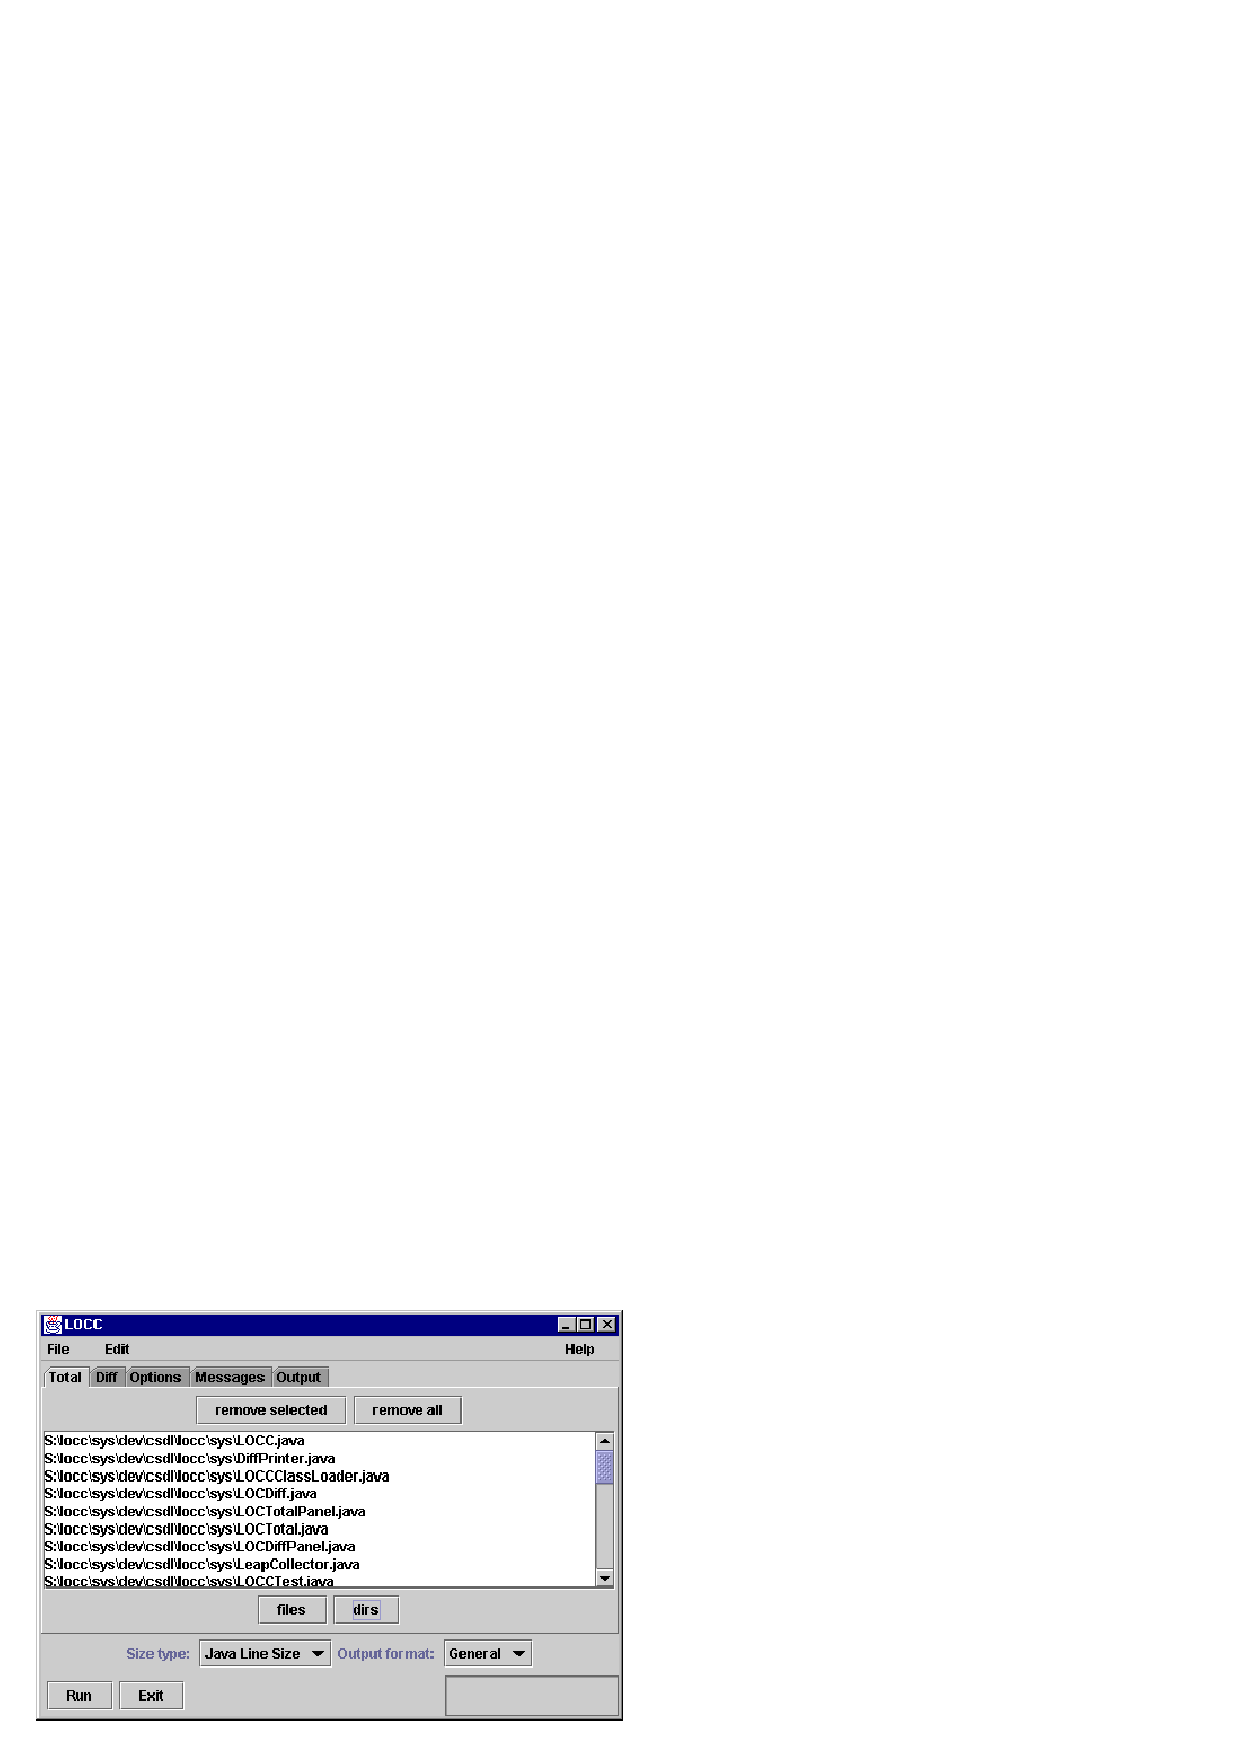
\includegraphics[angle=-90,width=\textwidth]{figs/total-panel.epsi}
  \caption{LOCC's total size counting panel}
  \label{fig:total-panel}
\end{figure}

This panel, shown in Figure \ref{fig:total-panel}, provides methods by which the developer can add files to
the list of files to be counted in total.  The ``files'' button allows 
files to be added one at a time.  The ``dirs'' button allows an entire 
directory to be added, or those files in a directory matching a
particular pattern.  Additional buttons allow the user to selectively
remove files from the list, or to clear the list entirely.  Identical
functionality can be accessed via the menu bar.

\subsection{Diff Panel}

\begin{figure}
%  \vspace{3.5in}
  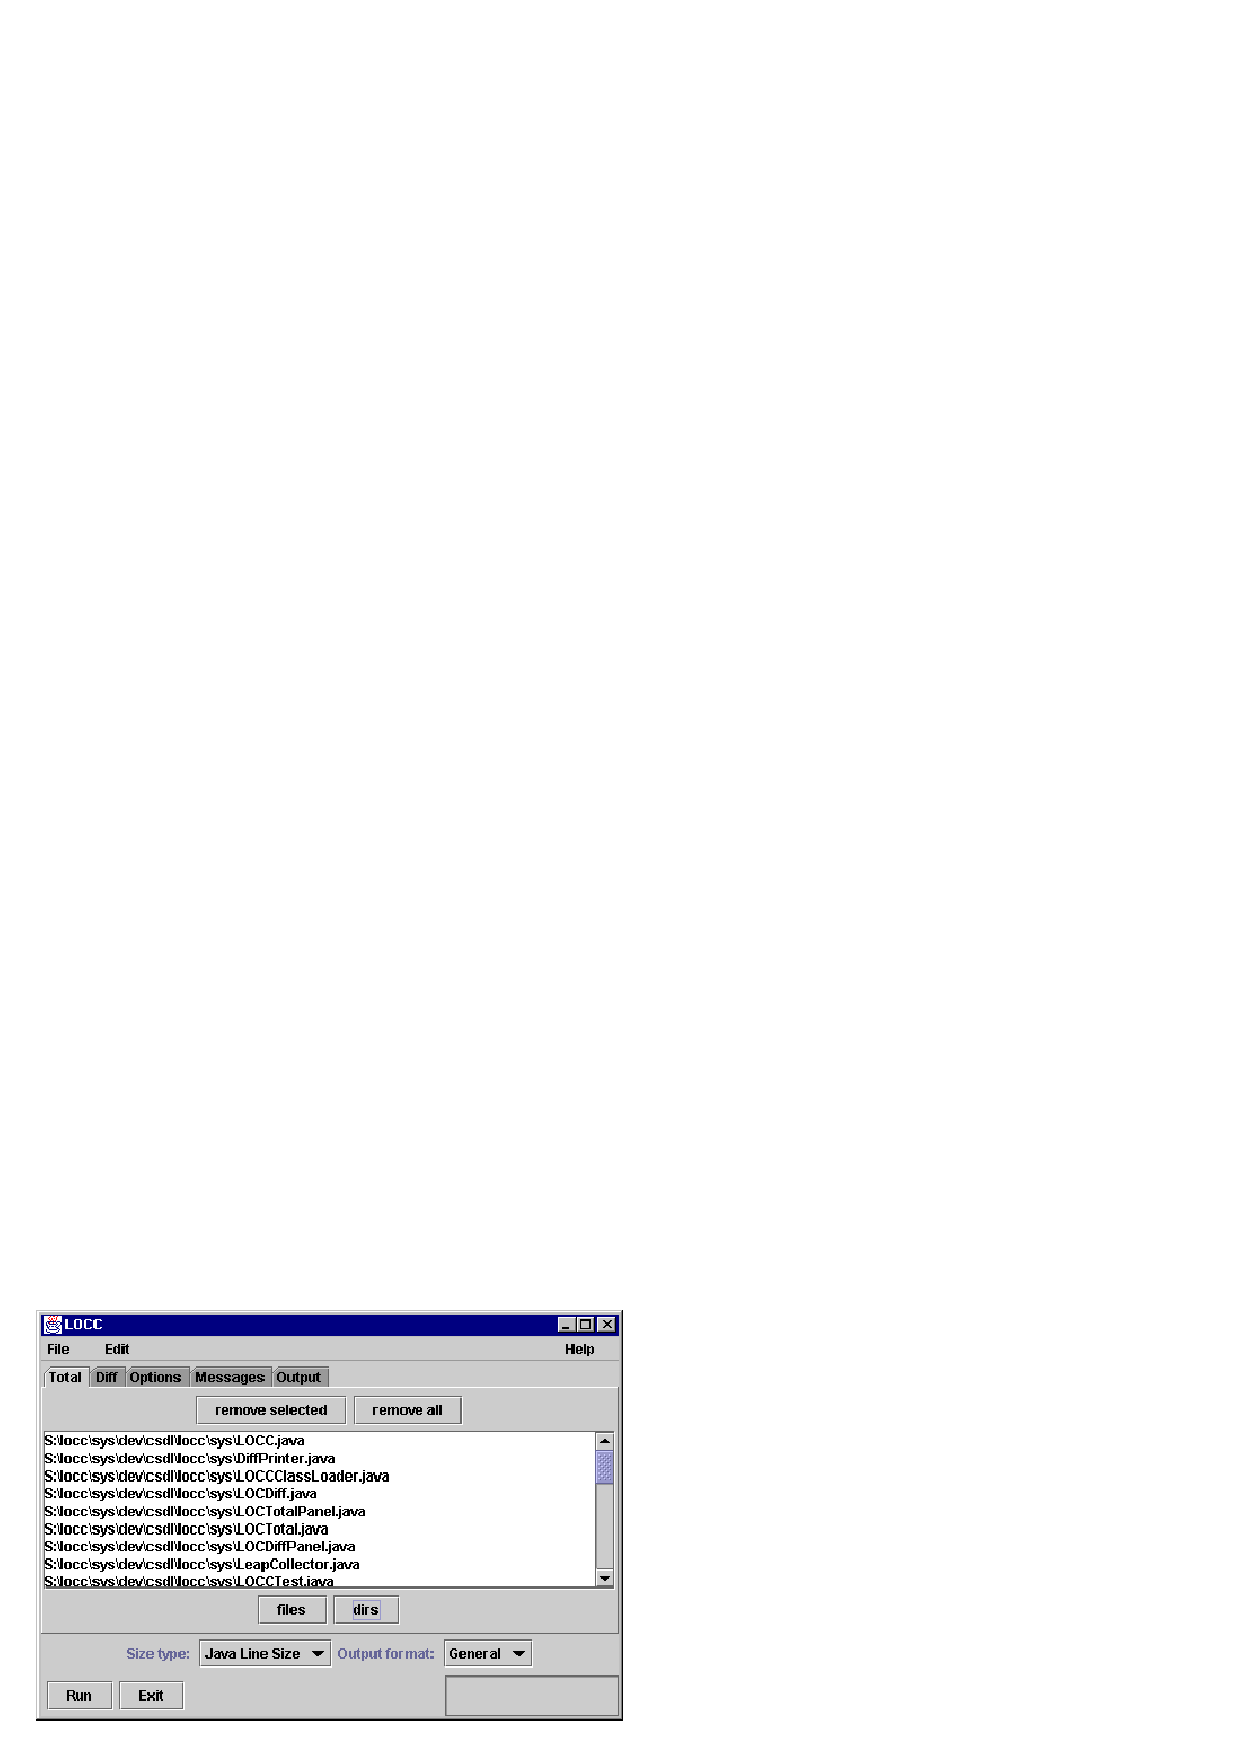
\includegraphics[angle=-90,width=\textwidth]{figs/total-panel.epsi}
  \caption{LOCC's size difference counting panel}
  \label{fig:diff-panel}
\end{figure}

This panel allows the user to specify the file pairs which will be
compared in a difference operation.  The user must specify both the old
and new versions of the file.  There are again two ways to do this.
The ``files'' button will bring up a dialog which will allow the user
to directly select the two files.  The ``dirs'' button will bring up a 
dialog which will allow the user to specify two directories and a file 
extension.  The directories containing the original file versions and
the new file versions will be called the ``old'' and ``new''
directories, respectively. 

Processing proceeds as follows.  All files in the old directory which
match the chosen extension (all files ending in ``.java'', for
instance) are collected in a list.  Then a list of all files in the
new directory is obtained and sorted.  For each file in the old
directory list, a search is made in the new directory.  For each
successful search, a pair of files is added to the list of pairs to be 
counted.  Both the sort and the search are implemented in such a way
that even large directories should be processed fairly quickly.

Like the total panel, the diff panel has buttons to remove file pairs, 
and to clear the list of file pairs.

\subsection{Output Options}

\begin{figure}
%  \vspace{3.5in}
  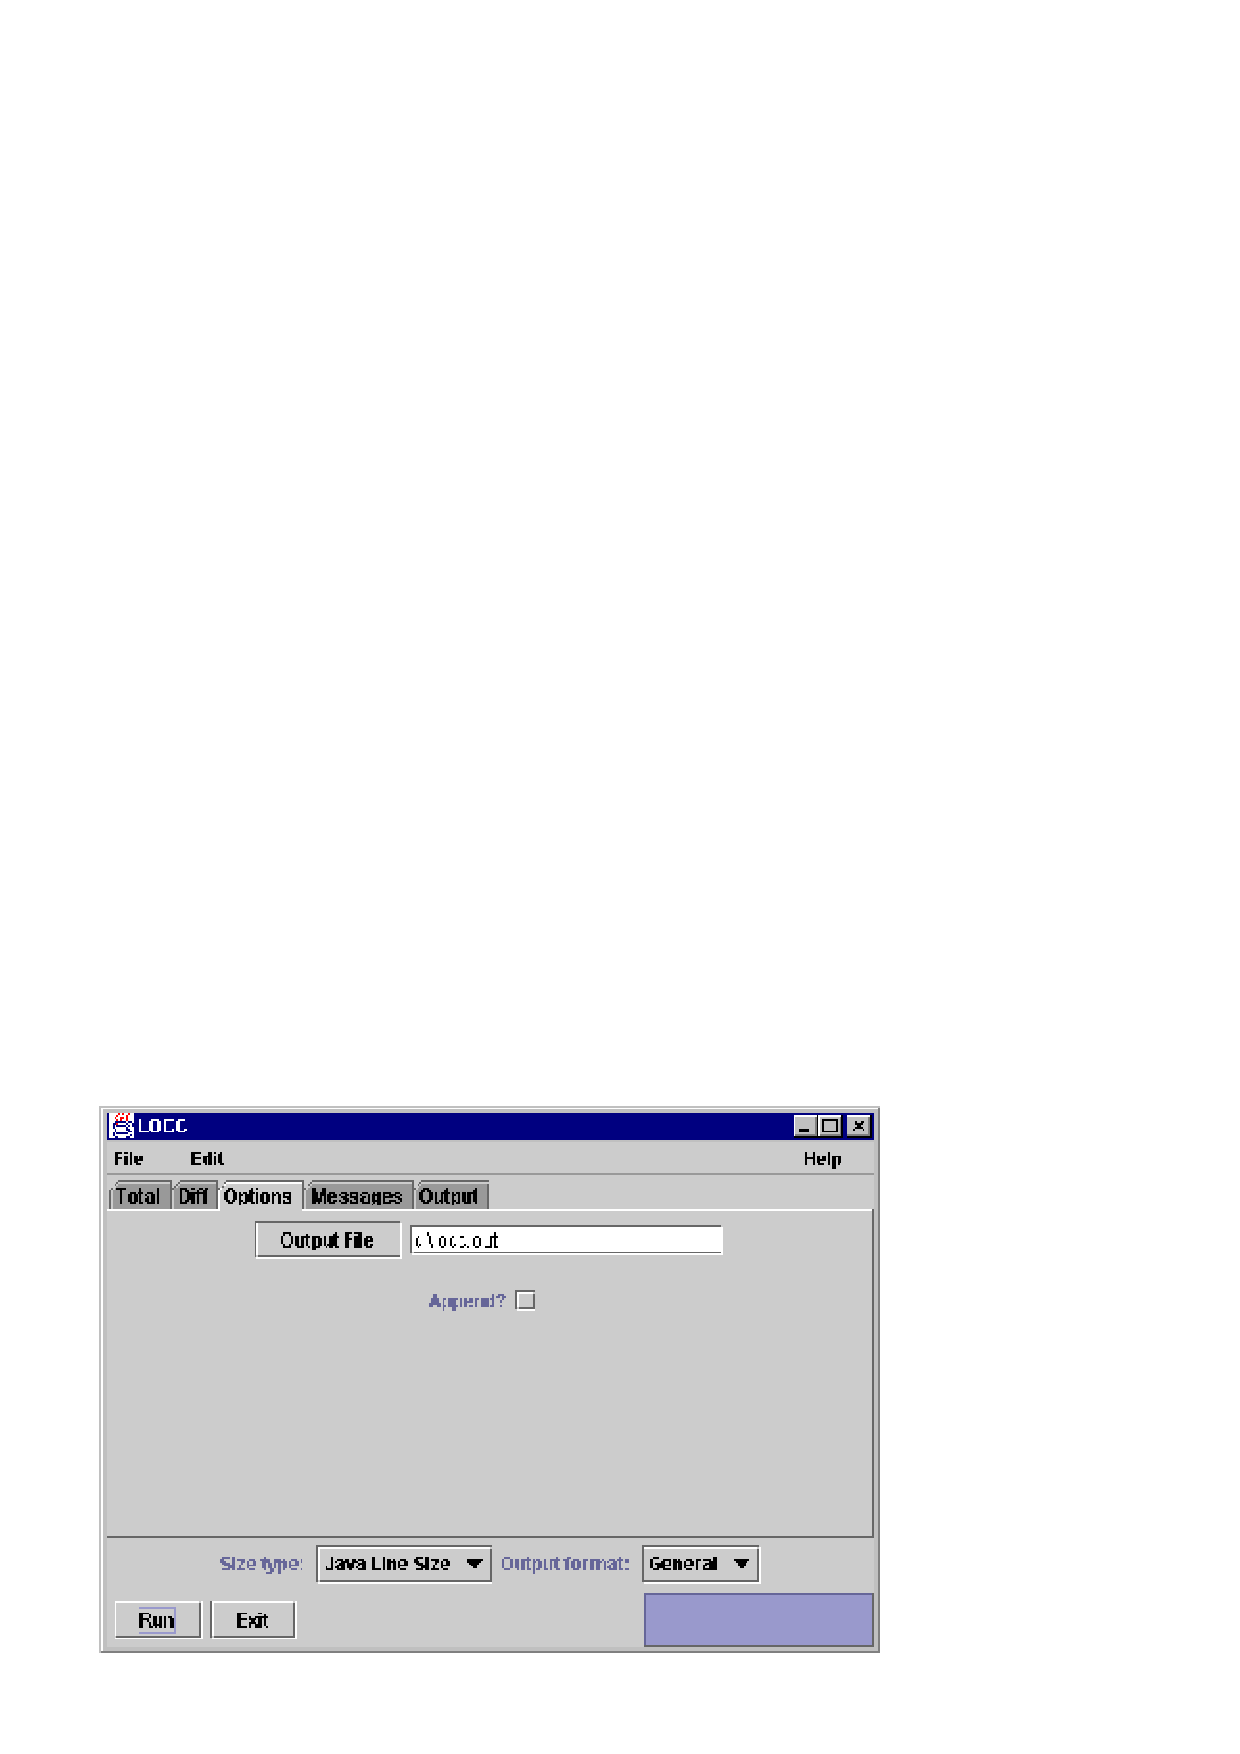
\includegraphics[angle=-90,width=\textwidth]{figs/options-panel.epsi}
  \caption{LOCC's options panel}
  \label{fig:options-panel}
\end{figure}

The output options panel allows the user to select a file in which to
place the output of the counts.  The file name can be typed directly
into the text field, or the button can be pressed to activate a file
chooser.  A check box allows the user to select overwrite or append
mode when writing to the file.

\subsection{Messages}

\begin{figure}
%  \vspace{3.5in}
  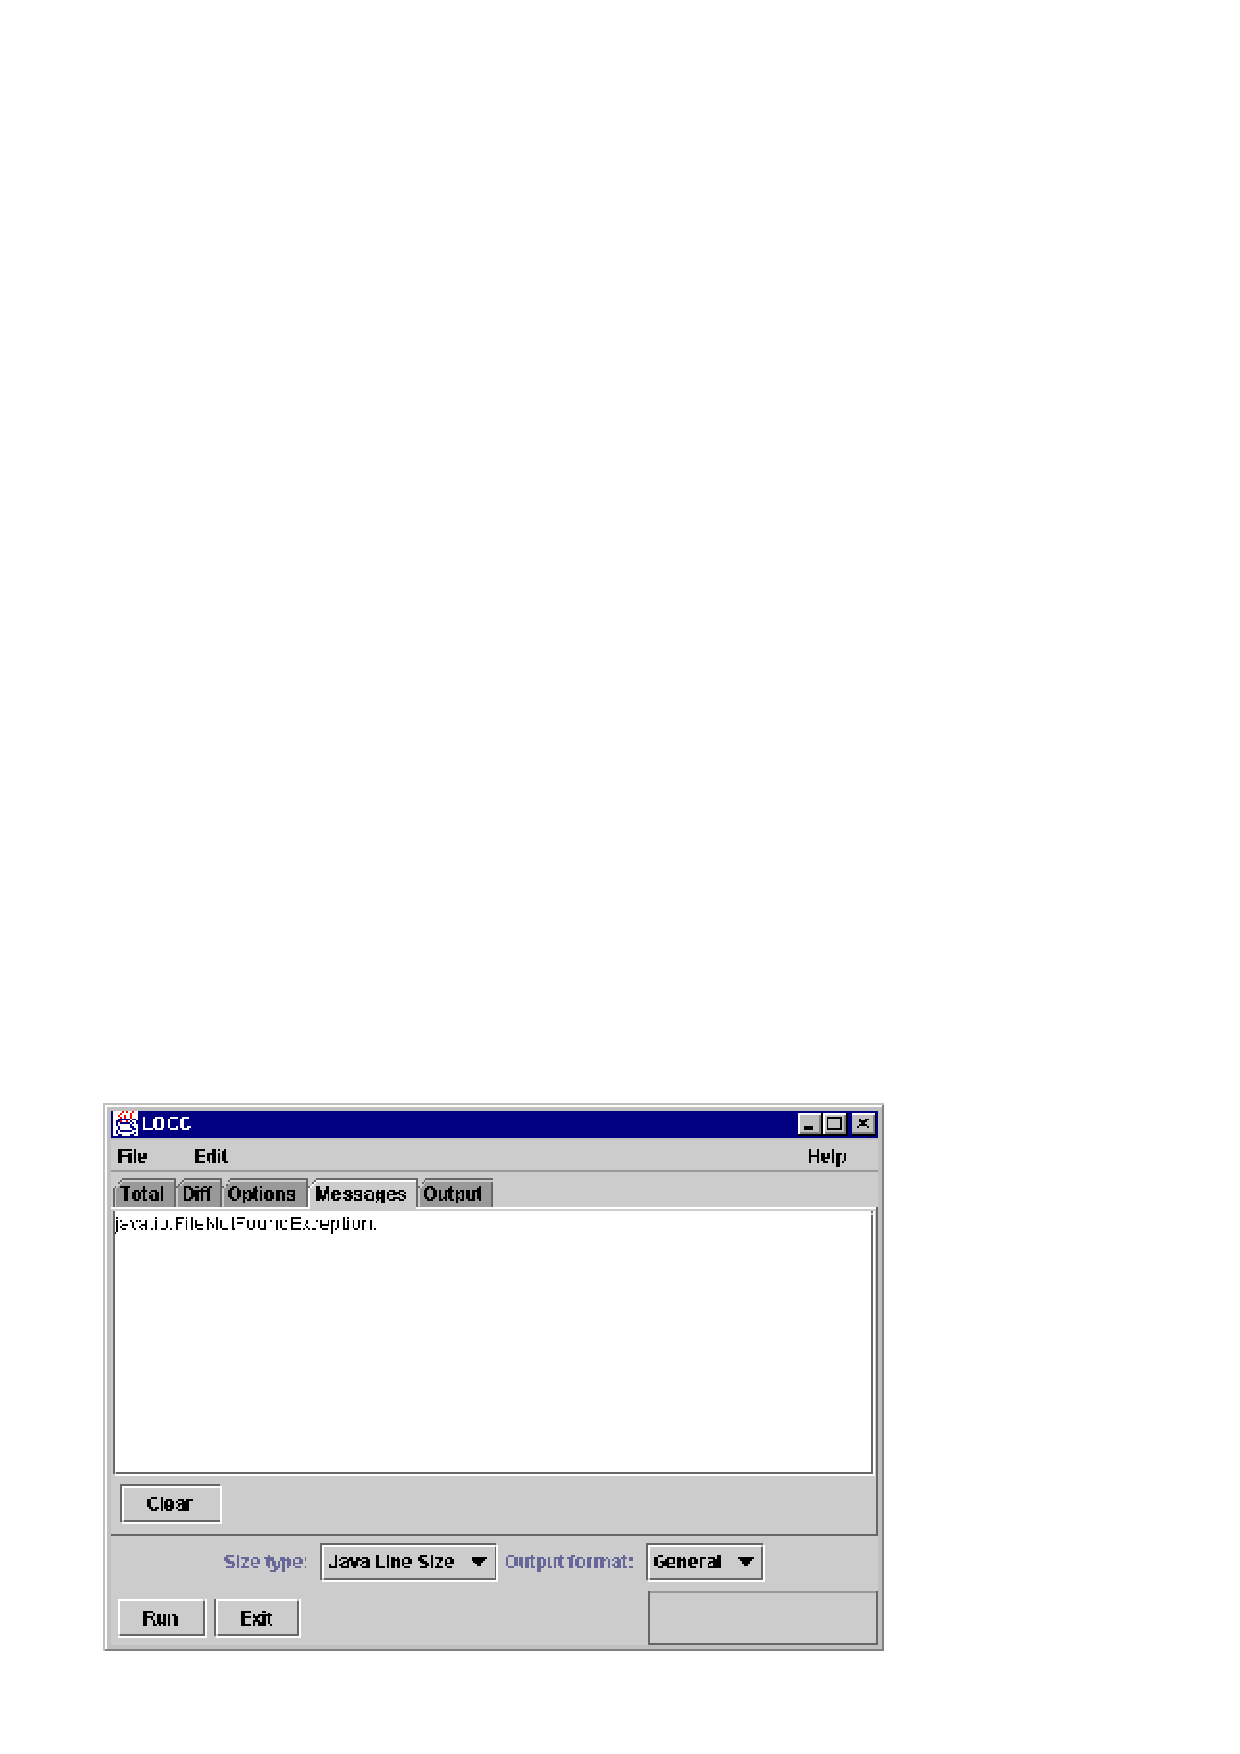
\includegraphics[angle=-90,width=\textwidth]{figs/message-panel.epsi}
  \caption{LOCC's message panel}
  \label{fig:message-panel}
\end{figure}

The message panel contains error and warning messages generated when
producing the count.  These error messages may be ``procedural'',
e.g. the user specified an output file for which he does not have write
permission, or ``operational'', e.g. some event occurred which
prevented LOCC from counting a file.  The most common operational
error is a parse error when using a metric which includes a
parser.  LOCC provides a simple mechanism for authors of size metrics 
to produce error messages which will be displayed in the message
panel.

\subsection{Output}

\begin{figure}
%  \vspace{3.5in}
  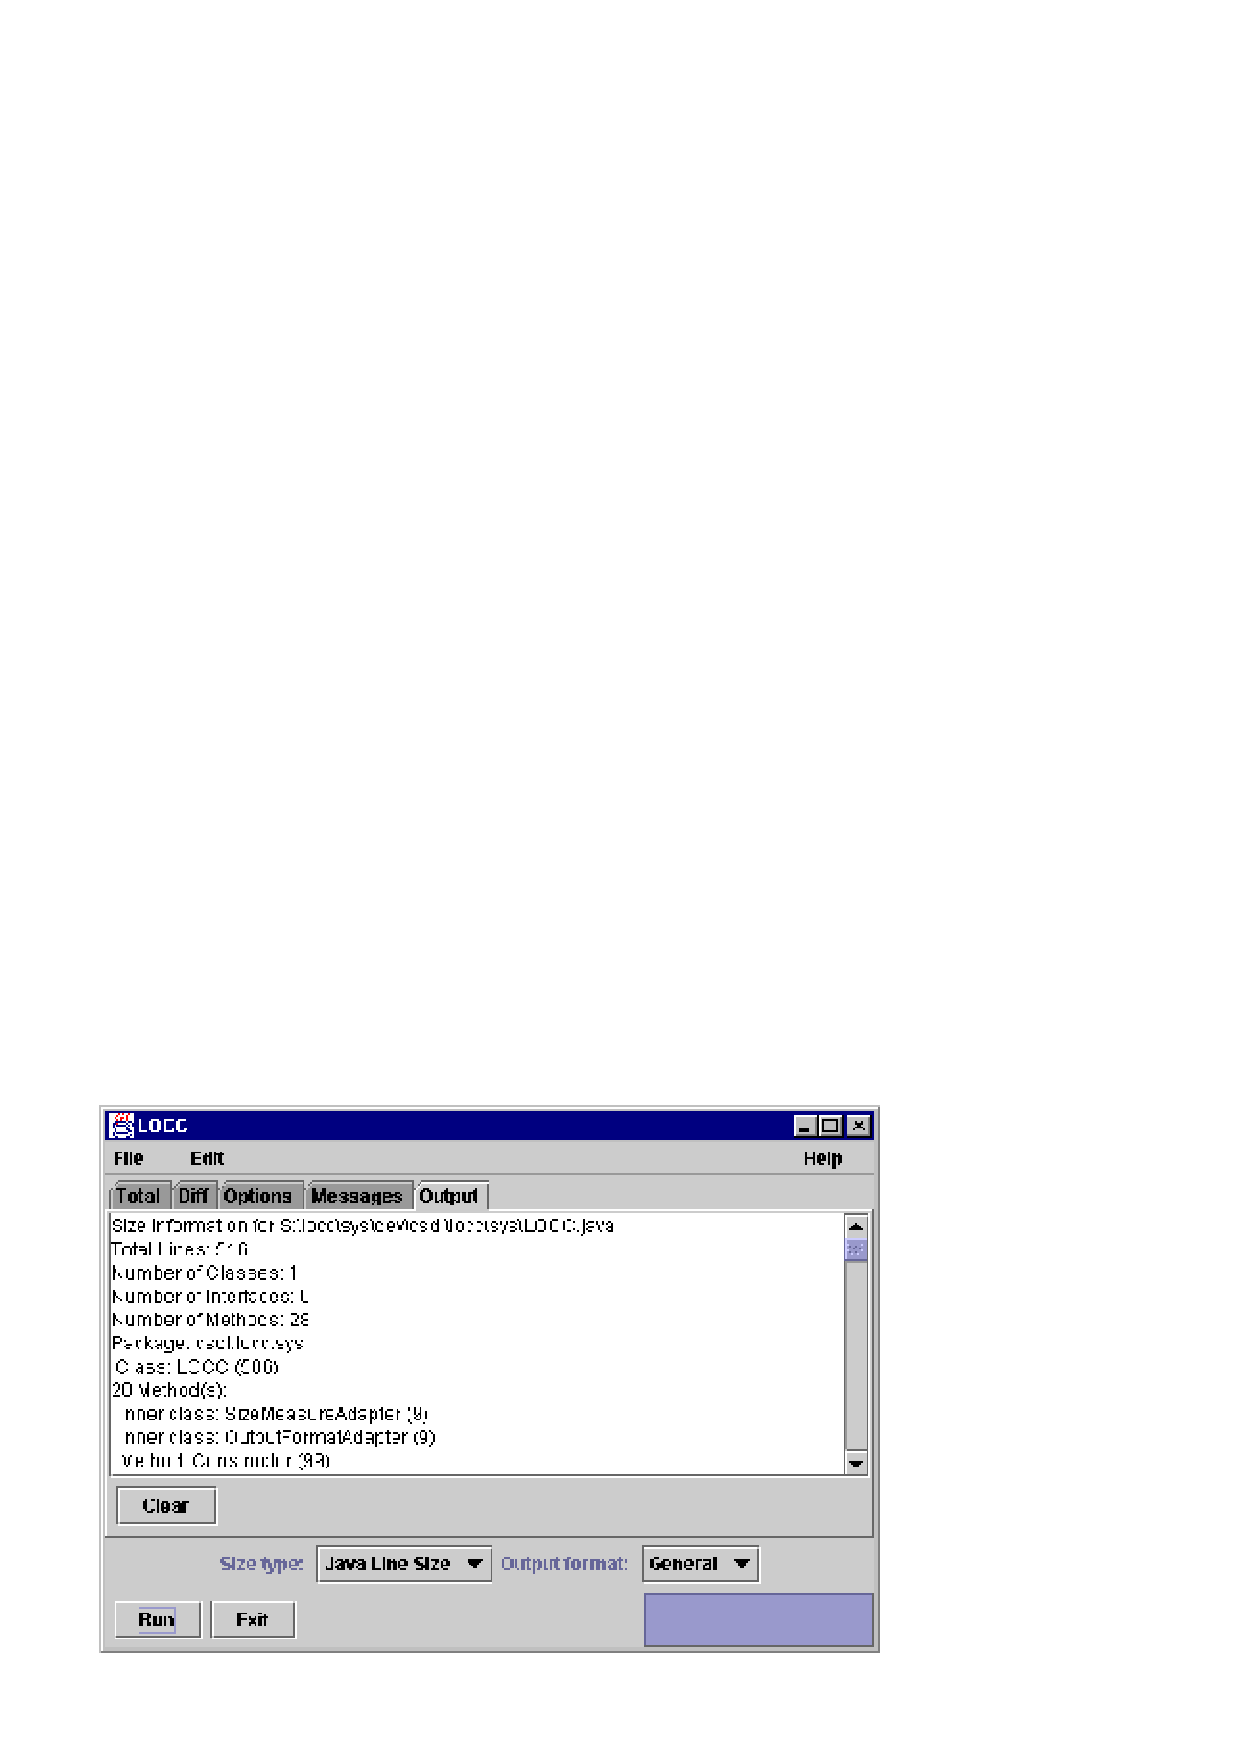
\includegraphics[angle=-90,width=\textwidth]{figs/output-panel.epsi}
  \caption{LOCC's output panel}
  \label{fig:output-panel}
\end{figure}

The output panel captures output from the running size operation.
Output may additionally be sent to a file, as specified in the output
options panel.  

\subsection{Running LOCC}

The user begins a session with LOCC by double clicking the mouse on
the icon given to LOCC when it was installed.  The LOCC GUI can also
be invoked from a command line, with the command 
\begin{verbatim}    java csdl.locc.sys.LOCC\end{verbatim}  

Once LOCC is running, the user will add the files to be counted in
total to the total panel, and the file pairs to be compared to the
diff panel.  If output to a file is desired, it should be specified in 
the output options panel.  The size type is selected from the pull down 
list, and the output format from a corresponding list.  The user then
clicks the ``Run'' button, and the processing begins.  Error
conditions will produce a dialog directing the user to the message
panel.  

\section{Using the command line interface}

The command line interface is not intended to be the primary interface 
for users of LOCC, but is available, e.g. so that users who wish to
use LOCC from within a script can do so.  There are separate commands
to invoke total and diff counting.  

\subsection{Total counting}

The syntax for the command line for total counting is

\begin{verbatim}    java csdl.locc.sys.LOCTotal [options]\end{verbatim}

where {\tt [options]} can be any of the following:

\begin{itemize}

\item {\tt -sizetype} {\em metric} : this option tells LOCC which size
      metric to use.  If {\em metric} is not specified, or if an
      invalid metric is given, a list of
      available size metrics will be printed.

\item {\tt -outformat} {\em format} : this option tells LOCC which output
      format to use for the given size metric.  If no output format is 
      given, or if an invalid output format is given, then available
      output formats for the given size metric will be listed.

\item {\tt -outfile} {\em file} {\tt | -} : the {\tt -outfile} option specifies
      the name of the file in which to send output.  If a single dash
      (``{\tt -}'') is given, then output is directed to standard output.
      If this option is not given, the default behavior is to produce
      a distinct output file for each input file, with name generated
      from the input file name with ``.siz'' appended.
        
\item {\tt -outdir} {\em dir} : this option, if given, directs LOCC to
      produce output files in the given directory.

\item {\tt -infiles} {\em file1 file2 \ldots} : this option specifies a list
      of files to count.  This option can be given more than once with the
      result that the file names from all {\tt -infiles} options are
      concatenated. 

\item {\tt -indir} {\em dir ext} : the {\tt -indir} option tells LOCC to
      count all the files in {\em dir} with file extension {\em ext}.
      A wildcard character is not needed, so the user would specify
      ``{\tt .java}'' instead of ``{\tt *.java}'', which would be
      expanded by the shell anyhow.

\end{itemize}

\subsection{Diff counting}

The syntax for the command line for diff counting is 

\begin{verbatim}    java csdl.locc.sys.LOCDiff [options]\end{verbatim}

where {\tt [options]} can be any of the following:

\begin{itemize}

\item {\tt -difftype} {\em metric} : {\em metric} is the name of the size
      metric to use in producing the diff.  If this option is not
      given, or if an invalid metric is named, a list of valid metrics 
      will be printed.

\item {\tt -outformat} {\em format} : this option tells LOCC which output
      format to use for the given size metric.  If no output format is 
      given, or if an invalid output format is given, then available
      output formats for the given size metric will be listed.

\item {\tt -new} {\em file} : {\em file} is the name of the new version of
      the file.

\item {\tt -old} {\em file} : {\em file} is the name of the old version of
      the file.

\item {\tt -outfile} ( {\em file} {\tt | -} ) : the {\em -outfile} option specifies
      the name of the file in which to send output.  If a single dash
      (``{\tt -}'') is given, then output is directed to standard
      output.  
              
\end{itemize}

Notice that while LOCTotal can count any number of files in one
invocation, LOCDiff can only process one file pair at a time.
